\chapter{Results} \label{chap:results}

In this chapter, we analyze the accuracy of our method for constrained spectral uplifting. We start by focusing on the effects of various implementation details on the results and justifying our decisions regarding their selection. Afterward, we present the actual results achieved in the form of rendered images, and analyze them in terms of their colorimetric properties.

We conclude this chapter by shortly overviewing the performance of our method by providing measurements of both memory utilization and time performance, and proposing improvements for future work.

\section{Implementation choices}

The structure of the trigonometric moment cube resulting from the implemented Borgtool's extension greatly depends on the choice of techniques and parameter values used during the implementation. To be specific, the core elements affecting the accuracy include:
\begin{itemize}
	\item the signal mapping technique used for spectral representation with trigonometric moments
	\item the number of trigonometric moments with which to store spectra
	\item the utilization of the optimizer, specifically its definition of residual blocks
\end{itemize}

This sections overviews our decision-making process regarding these issues, and presents results achieved with other methods to support our claim.

\subsection{Signal mapping techniques} \label{sec:storingMoments}
The first thing we analyze and decide on is the technique used for mapping wavelengths to a signal for the storage and subsequent reconstruction of moments. As already mentioned in~\cref{par:spectrumToCoefficientConversion}, we have the choice of both mirroring and warping the signal, which overall creates four options --- using only mirroring, using only warping, using both or using neither, i.e. utilizing the original signal.

Note that our requirements for the resulting spectral shapes differ depending on the type of the lattice point. For the atlas lattice points, we aim for the highest possible precision in terms of curve reconstruction, so as to lose as little information about the original atlas entry as possible. Regular lattice points, however, do not have a prior atlas entry that their spectra must approximate. Therefore, in order to prevent color artifacts upon interpolation, we mainly aim for their smoothness.

In addition to the reconstructed shape, we must also take the behavior of the optimizer (i.e. how well it improves upon its prior coefficients under the given signal mapping technique) into account.

We start by focusing on the accuracy of the reconstruction of atlas lattice points. We run an experiment across multiple color atlases (specifically the Pantone Color System, Munsell Book of Colors and the Macbeth Color Checker SG) and multiple CIE illuminants in which we compare the average and maximum round-trip errors of spectra under illuminants for all four techniques. Due to its continuous nature, we use the Delta E as the error measure.

In~\cref{sec:completeMomentError}, we provide all results obtained from these experiments. Note that using $n$ moments requires storing $n+1$ values in case mirroring is used (i.e. the moments are real) and $2n+1$ values otherwise (i.e. the moments are complex). As, from the implementation point of view, we are interested in the number of $coefficients$ needed for storage (i.e. the number of $double$ values per lattice point) rather than the number of moments, we surmise the contents of~\cref{sec:completeMomentError} in~\cref{table:comparisonMomentTechnique}, where we present the obtained errors according to the number of coefficients.

\begin{table}[t]
	\centering
	\begin{tabular}{crrrrrrrr}
		\toprule
		\multirow{4}{*}{Coefficients} &
		\multicolumn{8}{c}{Methods} \\
		\cmidrule(lr){2-9}
		&\multicolumn{2}{c}{M\&W} &
		\multicolumn{2}{c}{M\&nW} &
		\multicolumn{2}{c}{nM\&W} &
		\multicolumn{2}{c}{nM\&nW}\\
		\cmidrule(lr){2-9}
		& Avg & Max & Avg & Max & Avg & Max & Avg & Max \\
		\cmidrule(lr){1-9}
		1&23.88&130.27&23.95&130.62&23.86&130.38&23.95&130.62\\
		2&13.09&97.76&16.92&107.23&\textemdash&\textemdash&\textemdash&\textemdash\\
		3&1.39&21.71&10.18&74.62&4.08&51.23&8.48&67.12\\
		4&0.74&7.43&6.3&60.36&\textemdash&\textemdash&\textemdash&\textemdash\\
		5&0.49&5.46&2.58&26.36&1.31&20.87&2.56&20.14\\
		6&0.35&3.95&1.1&6.83&\textemdash&\textemdash&\textemdash&\textemdash\\
		7&0.31&3.19&0.73&6.12&0.71&8.18&0.89&6.36\\
		8&0.28&2.85&0.71&5.67&\textemdash&\textemdash&\textemdash&\textemdash\\
		9&0.27&2.42&0.61&3.94&0.61&5.16&0.46&3.62\\
		10&0.21&2.41&0.43&3.78&\textemdash&\textemdash&\textemdash&\textemdash\\
		11&0.21&2.41&0.26&2.62&0.47&4.11&0.37&3.2\\
		12&0.17&2.4&0.2&2.26&\textemdash&\textemdash&\textemdash&\textemdash\\
		13&0.17&2.39&0.2&2.32&0.32&3.07&0.27&2.73\\
		14&0.16&2.36&0.2&2.29&\textemdash&\textemdash&\textemdash&\textemdash\\
		15&0.16&2.32&0.2&1.93&0.29&2.28&0.24&2.26\\
		16&0.15&2.26&0.18&1.2&\textemdash&\textemdash&\textemdash&\textemdash\\
		17&0.15&2.23&0.17&1.17&0.29&1.89&0.23&1.52\\
		18&0.15&2.21&0.15&1.12&\textemdash&\textemdash&\textemdash&\textemdash\\
		19&0.15&2.19&0.14&1.12&0.27&1.8&0.19&1.1\\
		20&0.15&2.16&0.14&1.08&\textemdash&\textemdash&\textemdash&\textemdash\\
		\bottomrule
	\end{tabular}
	\caption{The average and maximum Delta E error originating from round-trips under various illuminants. $M$ represents mirroring, $W$ warping, and the symbol $n$ stands for their negation.}
	\label{table:comparisonMomentTechnique}
\end{table}

By observing~\cref{table:comparisonMomentTechnique}, we conclude that it is beneficial to mirror the signal. Although the non-mirroring technique performs slightly better for $c \le 9$, the input atlases often contain more complex spectra, where $c \le 9$ is insufficient. Additionally, the optimizer behaves similarly for both techniques, and therefore does not need to be accounted for.

By applying the same principle when choosing whether to warp the signal, we assume that warping should provide better results. We put this theory to practice and test the performance of the optimizer on the chosen technique. Specifically, our test includes storing atlas entries with a ``sufficient'' number of coefficients (sufficiency of a representation is determined by the round-trip Delta E error under FL11 illuminant as in~\cref{ssec:noOfMoments}) and using these coefficients as prior for the fitting of closest lattice points. The original and fitted curves are then compared.

Unfortunately, the results are unsatisfactory. Occasionally, the optimizer fails in so as the fitted curve does not follow the original at all but rather ends up as a spiky spectrum susceptible to metameric artifacts. We show some of these results in~\cref{fig:warping_atlasLatticePoints}.

Therefore, we resort to not warping the signal. Although the optimizer must process more coefficients than if the signal was warped (e.g. if seeding with the Munsell Book of Colors with the sufficiency conditions as in~\cref{ssec:noOfMoments}, $16$ coefficients are on average required for storing spectra, as opposed to $12$ if the signal is warped), the artifacts arising when warping the signal are completely eliminated (see~\cref{fig:warping_atlasLatticePoints}). In addition, the average distance between the original and fitted spectra is substantially lower.

\begin{figure}[t]
	\centering
	\captionsetup[subfigure]{font=footnotesize,labelfont=footnotesize}
	\captionsetup[subfigure]{justification=centering}
	\begin{subfigure}[t]{0.50\textwidth}
		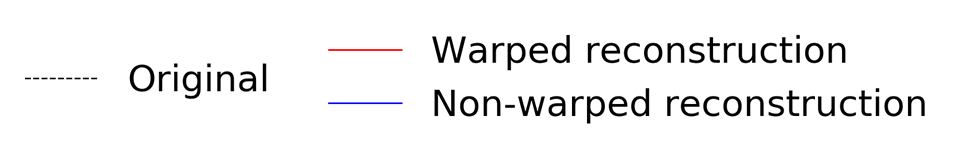
\includegraphics[width=\linewidth]{img/results_techniqueLegend.png}
	\end{subfigure} \\
	\begin{subfigure}[t]{0.32\textwidth}
		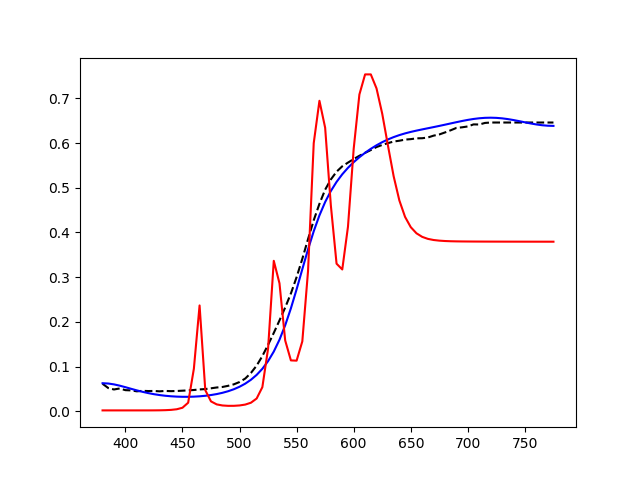
\includegraphics[width=\linewidth]{img/results_warping_orange.png}
		\caption{``orange'' patch}
		\label{fig:warping_alp_neutral50}
	\end{subfigure} \hspace{0.1em}
	\begin{subfigure}[t]{0.32\textwidth}
	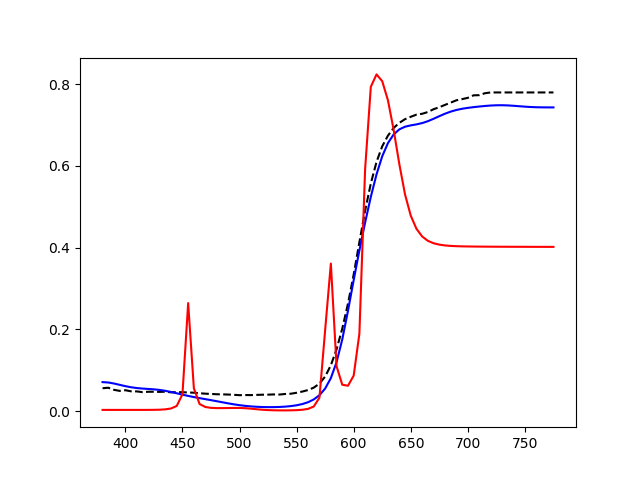
\includegraphics[width=\linewidth]{img/results_warping_red.png}
	\caption{``red'' patch}
	\label{fig:warping_alp_red}
	\end{subfigure} \hspace{0.1em}
	\begin{subfigure}[t]{0.32\textwidth}
		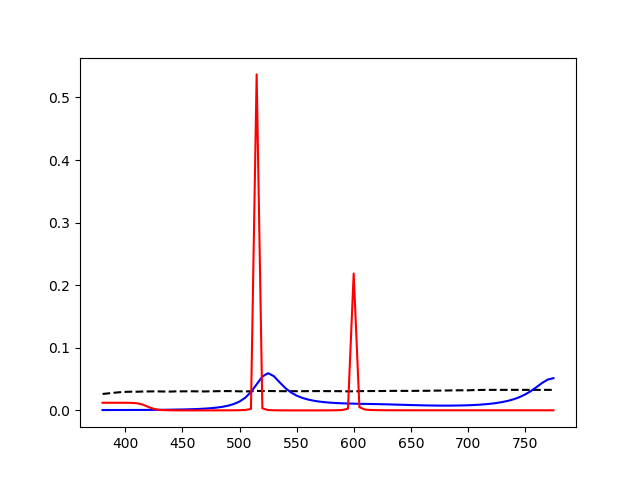
\includegraphics[width=\linewidth]{img/results_warping_black.png}
		\caption{``black'' patch}
		\label{fig:warping_alp_black}
	\end{subfigure}
	\caption{Failure of warping when fitting atlas lattice points, shown on patches from the Macbeth Color Chart}
	\label{fig:warping_atlasLatticePoints}
\end{figure}

For the regular lattice points, we present a similar comparison of these two methods in~\cref{fig:warping_regularPoints}, where we seed cubes of different sizes with distinct atlases and analyze the spectra at specific points. Not warping the signal is superior to warping even in this case, as it creates smoother spectra with less sharp edges. 

As we eventually decide on using only 3 coefficients per regular lattice points (see~\cref{ssec:noOfMoments}), and for that purpose, even warping works reasonably well, we do not necessarily need to account for regular lattice points when choosing whether to warp the signal. However, regardless, all the presented evidence points to the superiority of non-warping.

\begin{figure}[t]
	\centering
	\captionsetup[subfigure]{font=footnotesize,labelfont=footnotesize}
	\captionsetup[subfigure]{justification=centering}
	\begin{subfigure}[t]{0.38\textwidth}
		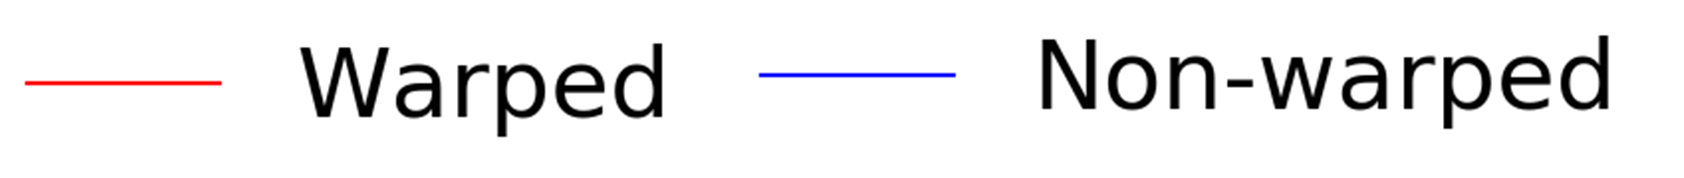
\includegraphics[width=\linewidth]{img/resultsTechniqueOpt_legend.png}
	\end{subfigure} \\
	\begin{subfigure}[t]{0.31\textwidth}
		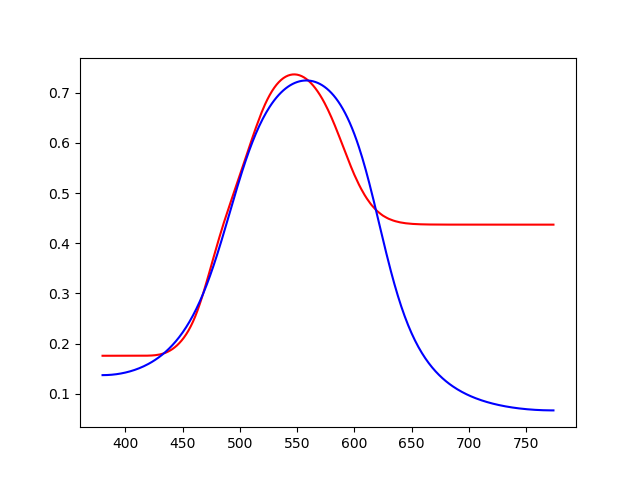
\includegraphics[width=\linewidth]{img/resultsTechniqueOpt_m3_cd64.png}
		\caption{$c=3, cd=64$,\\$RGB=(222.6, 230.7, 230.7)$,\\initial atlas = Macbeth Color Chart}
		\label{fig:warping_regularPointst_m3_cd64}
	\end{subfigure}
	\begin{subfigure}[t]{0.31\textwidth}
		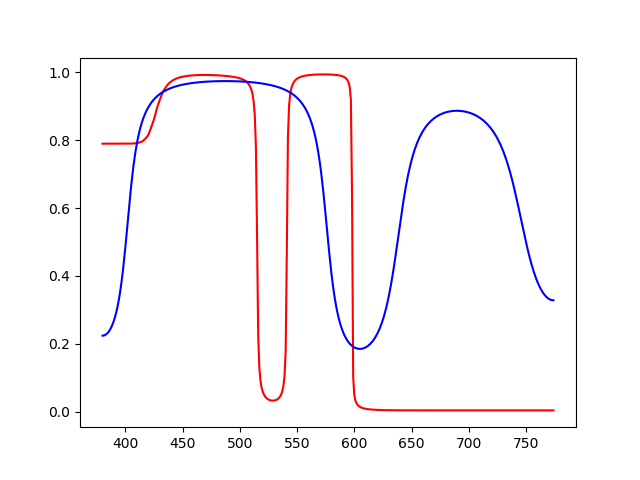
\includegraphics[width=\linewidth]{img/resultsTechniqueOpt_m5_cd32.png}
		\caption{$c=5, cd=32$,\\$RGB=(82.26, 172.74, 255)$,\\initial atlas = Page 14 from Munsell Book of Color}
		\label{fig:warping_regularPoints_m5_cd32}
	\end{subfigure}
	\begin{subfigure}[t]{0.31\textwidth}
		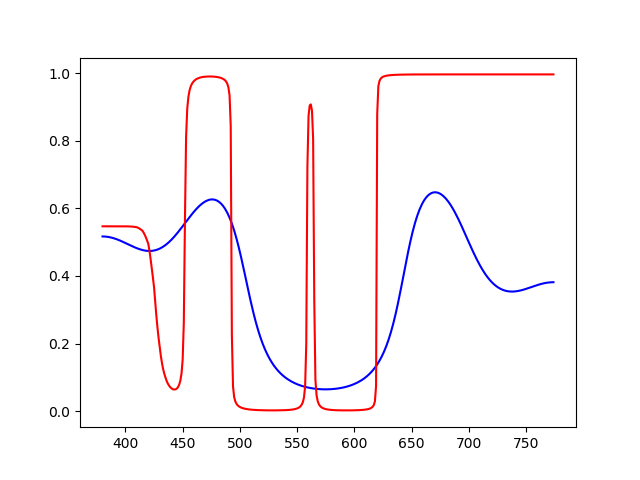
\includegraphics[width=\linewidth]{img/resultsTechniqueOpt_m7_cd16.png}
		\caption{$c=7, cd=16$,\\$RGB=(102, 17, 153)$,\\ fitted from middle}
		\label{fig:warping_regularPoints_m7_cd16}
	\end{subfigure} 
	\caption{Comparison of warping and non-warping when used for fitting regular atlas entries. Note that the figures are illustrative, as they were created with an older version of the cube and therefore may not correspond to the current results.}
	\label{fig:warping_regularPoints}
\end{figure}

To justify the failures of warping, we analyze its behavior during round-trips in comparison to that of not warping. In~\cref{fig:resultsWarping}, we present a few such examples on different curves with different number of coefficients. We can clearly observe the behavior for which warping was designated --- while the slight waves in the middle of the curve (at around 550nm) are reconstructed almost perfectly, the edges of the curve (i.e. the part of the curve leading up to 450nm and from 650nm) are flat and attain constant values.

Therefore, if warping the signal, the optimizer has very little influence on the edges of the curve. For that reason, it opts for optimizing only its middle, which might result in amplifying the already created sinusoidal-shapes.

By not warping the signal, on the other hand, the optimizer focuses on the spectra as a whole and is therefore less prone to spiky artifacts.

Therefore, we conclude that mirroring, but not warping the signal is the optimal approach for our purposes.

\begin{figure}[t]
	\centering
	\captionsetup[subfigure]{font=footnotesize,labelfont=footnotesize}
	\captionsetup[subfigure]{justification=centering}
	\begin{subfigure}[t]{0.60\textwidth}
		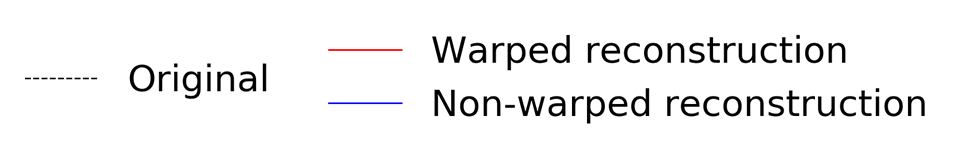
\includegraphics[width=\linewidth]{img/results_techniqueLegend.png}
	\end{subfigure} \\
	\begin{subfigure}[t]{0.45\textwidth}
		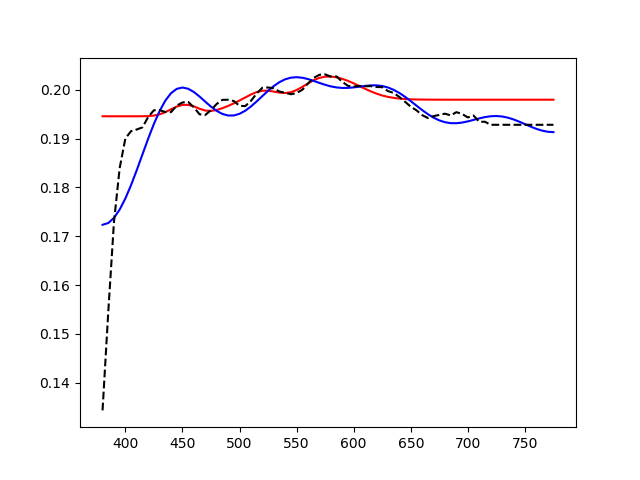
\includegraphics[width=\linewidth]{img/results_techniqueNeutral5.png}
		\caption{``neutral 5'' patch, $c = 9$}
		\label{fig:resultsWarping_neutral5}
	\end{subfigure} \hspace{0.1em}
	\begin{subfigure}[t]{0.45\textwidth}
		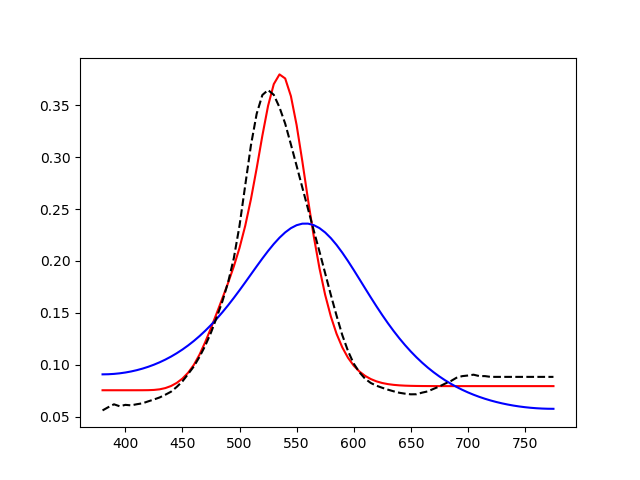
\includegraphics[width=\linewidth]{img/results_techniqueGreen.png}
		\caption{``green'' patch, $c = 3$}
		\label{fig:resultsWarping_green}
	\end{subfigure} \hspace{0.1em}
	\vspace{0.5em}\\
	\begin{subfigure}[t]{0.45\textwidth}
		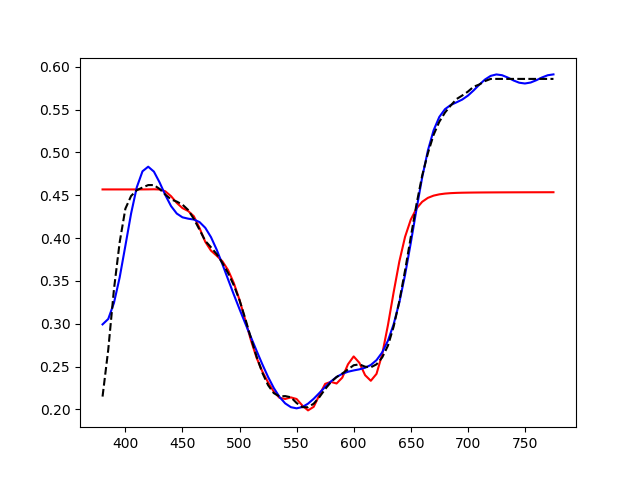
\includegraphics[width=\linewidth]{img/results_techniqueBlueFlower.png}
		\caption{``blue flower'' patch, $c = 16$}
		\label{fig:resultsWarping_blueFlower}
	\end{subfigure} \hspace{0.1em}
	\begin{subfigure}[t]{0.45\textwidth}
		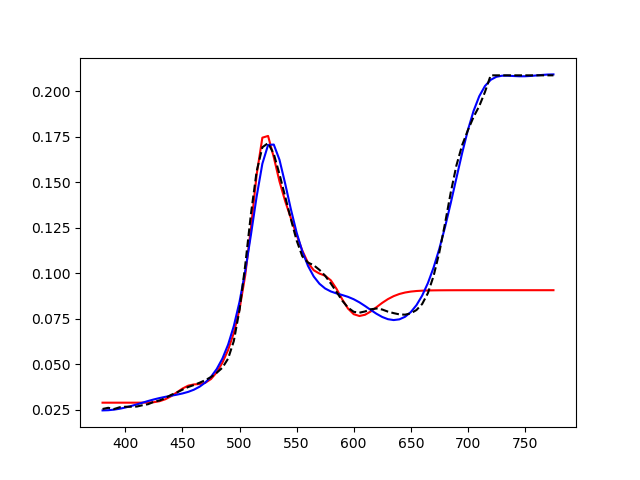
\includegraphics[width=\linewidth]{img/results_techniqueFoliage.png}
		\caption{``foliage'' patch, $c = 12$}
		\label{fig:resultsWarping_foliage}
	\end{subfigure}
	\caption{Comparison between the warped and non-warped reconstructed signal shown on multiple patches of the Munsell Book of Colors}
	\label{fig:resultsWarping}
\end{figure}

\subsection{Number of moments} \label{ssec:noOfMoments}

Another important parameter to determine is the number of moments (or coefficients) with which to store spectra at both atlas lattice points and regular lattice points.

We start by analyzing the atlas lattice points. Specifically, we focus on the number of coefficients with which to store atlas entries in the second step of our implementation (see~\cref{ssec:cubeSeeding}), as those are the coefficients that are then used as prior for atlas lattice points. Naturally, we wish for the reconstruction to be as precise as possible, however, we want to prevent unnecessarily high coefficient counts both to avoid high memory utilization and to simplify the run of the optimizer.

\begin{figure}[t!]
	\centering
	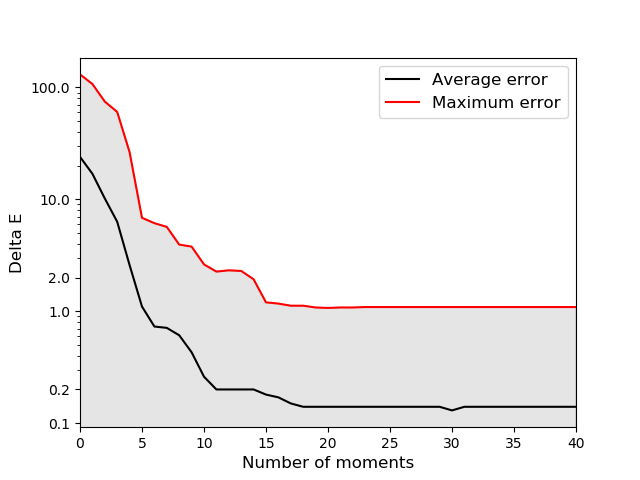
\includegraphics[width=0.6\linewidth]{img/results_noOfMoments_deltaE.png}
	\caption{The average and maximum Delta E error achieved by round-trips, surmised from~\cref{table:comparisonMomentTechnique}}
	\label{fig:results_noOfMoments_deltaE}
\end{figure}

By observing~\cref{fig:results_noOfMoments_deltaE}, we see that the Delta E error obtained by round-trips under the CIE illuminants stabilizes at $m=20$, i.e. $c=21$. As the curve precision does not worsen by adding more coefficients to the representation, storing all atlas entries with 21 coefficients might seem to be the optimal solution. Such approach is, however, wasteful for multitude of smooth, simple spectra.

Therefore, we decide to store each spectrum with only the necessary amount of coefficients. We obtain this number for each atlas entry iteratively --- starting from $c=4$, we check whether the coefficient count is sufficient, and, if not, we increase it and move on to the next iteration, repeating this process up to $m=21$.

We determine the sufficiency of a coefficient representation by picking one of the most error-prone illuminants and determining the round-trip error under said illuminant. If the error falls below a certain, pre-defined threshold, we declare the representation sufficient.

To determine which illuminant to use, we performed an experiment in which we computed the average number of coefficients required to achieve a specific error for a set of spectra. We then compared these values for all elements on the list of CIE illuminants (again excluding the E and D73 illuminants). By the assumption that these results give us a rough approximation of the average error, we concluded that the illuminant with the highest coefficient count is the most error-prone.

We present the results of our experiment in~\cref{table:sufficientCoefficientIlluminants}. We use an error of $\Delta E_{ab}^*=0.1$ due to the coefficient count variability under it, but any other would give similar results in terms of the order of the illuminants' coefficient counts.

Since the FL11 illuminant requires the highest number of coefficients, we use it for our purposes, and move on to examining the optimal threshold.

Surprisingly, utilizing the Delta E error in our iterative process of acquiring coefficients did not provide as satisfactory results as expected --- the entries represented with high number of coefficients ($c \ge 20$) were often unnecessarily accurate, while the entries represented with low number of coefficients ($c \le 10$) often lacked precision. Therefore, we decided to compute the error as an  absolute difference over all three RGB components, which outperformed both the Delta E error and even the Euclidean error in the RGB space (which was prone to similar, but less noticeable, behavior than the Delta E error). We set the threshold to $0.1$ for an RGB range of $(0,255)$, as we found it to perform well when tested for the actual uplifting. 

Although we attribute the failure of Delta E to its non-linearity, we have not yet obtained evidence as to support this claim.

Our approach for determining the sufficiency of coefficients is definitely not flawless. Firstly, neither the threshold, nor the computation of the error have been properly examined, which implies that there may be other, more suitable options. Secondly, since we examine only 18 CIE illuminants, there is a high chance that other, more error-prone, exist.

Even the assumption that the average coefficient count determines the worst-performing illuminant falls short. As we have come across multiple atlas entries that attain the highest color error under an illuminant other than FL11, checking whether the error satisfies the threshold for all illuminants might be a more effective approach.

Furthermore, even if we were to perfect our method, there exist a lot more, vastly different approaches that might be used. However, their exploration and analysis is not within the scope of this thesis, and, as our method produces reasonable results, we leave it for future work.

\begin{table}[t]
	\newcolumntype{?}{!{\vrule width 1.5pt}}
	\centering
	\begin{tabular}{c|c?c|c?c|c}
		\hline
		\rule{0pt}{5ex}
		Illuminant & \makecell{Average\\error} & Illuminant & \makecell{Average\\error}&Illuminant & \makecell{Average\\error}\\ 
		\hline
		\rule{0pt}{3ex}
		A & 14.8 & F & 12.91 & F7 & 12.55 \\ 
		B & 5.19 & F2 & 13.01 & F8 & 12.01 \\ 
		C & 16.11 & F3 & 12.93 & F9 & 12.09 \\ 
		D50 & 15.56 & F4 & 12.98 & F10 & 16.24 \\ 
		D65 & 15.64 & F5 & 12.95 & F11 & 16.46 \\ 
		D75 & 15.76 & F6 & 13.08 & F12 & 16.30 \\ 
		\hline
	\end{tabular}
	\caption{The average number of coefficients needed to achieve a round-trip error of $\Delta E_{ab}^* = 0.1$ for different CIE illuminants}
	\label{table:sufficientCoefficientIlluminants}
\end{table}

Finding the sufficient coefficient count for regular lattice points is a lot more straightforward than for the atlas lattice points. We remind that the only requirement is for the spectra to be smooth, so as to avoid interpolation-caused artifacts. This property is especially important if two significantly different, spiky atlas entries are fitted in voxels close to each other. Propagating their original shapes during the cube fitting process would, under a different illuminant, create a noticeable color boundary, which is undesired.

Figure~\cref{fig:warping_regularPoints} already suggests that using less coefficients might benefit our smoothness requirement. We put this theory to test by comparing spectra of regular lattice points fitted with a different number of coefficients in cubes of otherwise identical parameters. We present some of the results in~\cref{fig:noOfMoments_regularPoints}.

\begin{figure}[t]
	\centering
	\captionsetup[subfigure]{font=footnotesize,labelfont=footnotesize}
	\captionsetup[subfigure]{justification=centering}
	\begin{subfigure}[t]{0.60\textwidth}
		
\includegraphics[width=\linewidth]{img/results_noOfMoments_regularPts_legend.png}
	\end{subfigure} \\
	\begin{subfigure}[t]{0.45\textwidth}
		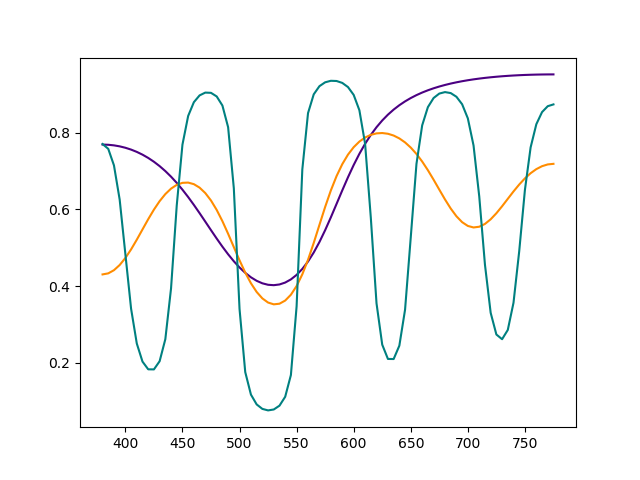
\includegraphics[width=\linewidth]{img/results_noOfMoments_regularPts_1.png}
		\caption{$RGB=(222.1, 106.9, 164.5)$,\\ fitting round $= 8/17$}
	\end{subfigure}
	\begin{subfigure}[t]{0.45\textwidth}
		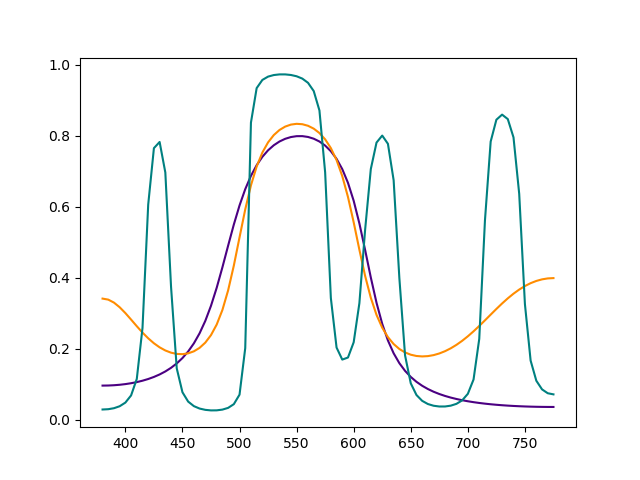
\includegraphics[width=\linewidth]{img/results_noOfMoments_regularPts_2.png}
		\caption{$RGB=(98.7, 205.6, 41.1)$,\\ fitting round $= 9/17$}
	\end{subfigure} 
	\caption{The effects of various choices for the regular lattice points' coefficient count on the shape of their spectra.}
	\label{fig:noOfMoments_regularPoints}
\end{figure}

Our assumptions have proven to be correct. By using less coefficients, we limit the optimizer's ability to reconstruct complicated spectra, therefore forcing it to create smooth, simple shapes. Specifically, we decide on using 3 coefficients --- as their shapes are sufficient, using more is unnecessary, but 2 were unable to recreate shapes and occasionally ended up reconstructing constant, straight lines.

Additional benefit of using only 3 coefficients per regular lattice point (as opposed to using a higher number) is the lower run-time of cube fitting, as well as less optimizer failures and therefore no need for invocation of heuristic improvements.

\subsection{Cost functions} \label{ssec:costFunctions}

In addition to the moment storage technique, another thing greatly affecting the outcome of the fitting are the cost functions of optimizer.

For the fitting of the sigmoids, Borgtool uses three cost functions, or \emph{residuals}, each of them specifying the absolute color difference in one axis of the RGB cube. Such an approach outperforms both the Euclidean color distance and even the Delta E difference --- the higher the number of meaningful residuals, the more information can the optimizer deduce about the coefficients' behavior, which, in turn, results in faster and more precise convergence.

As this approach performs rather decently in terms of both time complexity and the obtained results for the sigmoids, we try it out for the purposes of our optimization as well. 

In case of fitting of the regular lattice points (see~\cref{ssec:cubeFitting}), the obtained results are satisfactory, both for the fitting in the second round (i.e. after the ``recalculation'') and in the latter rounds (see~\cref{fig:costFunctionsRegularFitting}). The resulting curves are smooth, they evaluate to the desired RGB values, and the run-time is even better than for the sigmoids. Therefore, for the regular lattice points, we utilize this approach.

\begin{figure}[t]
	\centering
	\begin{subfigure}[t]{0.4\textwidth}
		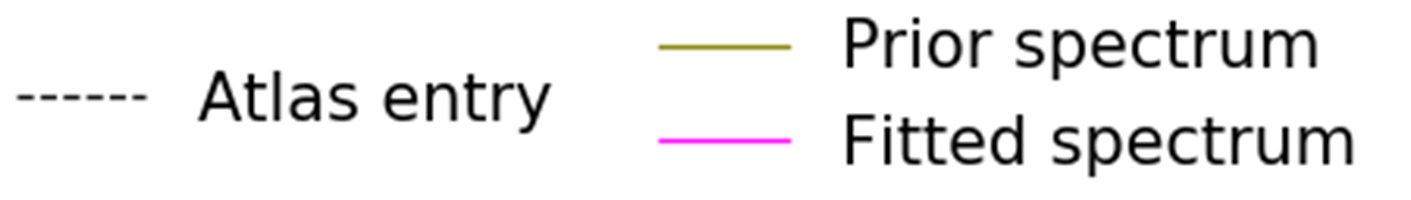
\includegraphics[width=\linewidth]{img/cost_functions_regular_legend.png}
	\end{subfigure} \\
	\begin{subfigure}[t]{0.45\textwidth}
	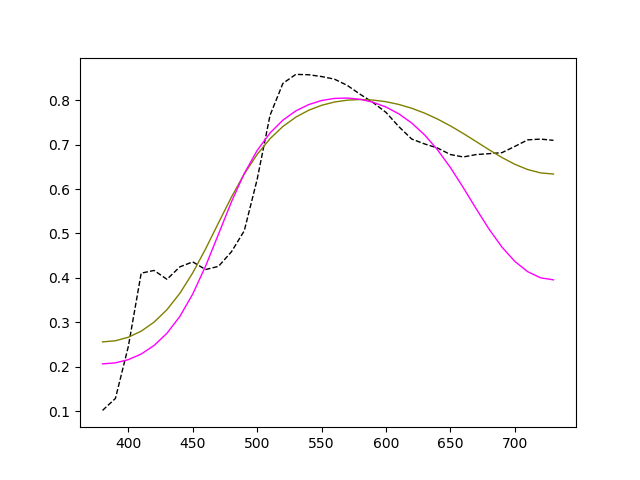
\includegraphics[width=\linewidth]{img/cost_functions_regular_round2.png}
	\caption{Fitting in the second round, i.e. the prior coefficients are the result of ``recalculation'' of the fitted coefficients of an atlas lattice point}
	\label{fig:costFunctionsRegularRound2}
	\end{subfigure} \hspace{0.1em}
	\begin{subfigure}[t]{0.45\textwidth}
		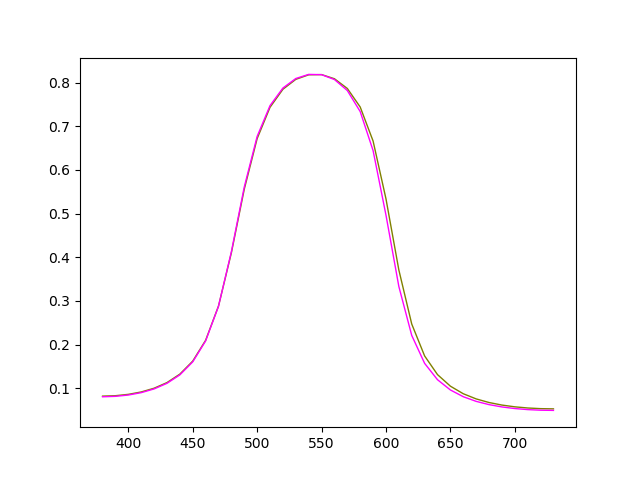
\includegraphics[width=\linewidth,height=0.2\textheight]{img/cost_functions_regular_round8.png}
		\caption{Fitting in round 8/20, where the prior spectrum is that of a regular lattice point}
		\label{fig:costFunctionsRegularRound8}
	\end{subfigure} 
	\caption{Fitting of regular lattice points with 3 RGB cost functions}
	\label{fig:costFunctionsRegularFitting}
\end{figure}

However, for fitting the atlas lattice points, this method is unsatisfactory. Although it terminates as successful (as the RGB of the resulting curve is within the fitting threshold of the target RGB), the reflectance curve takes on a sinusoidal shape with a rather high amplitude, therefore losing resemblance to the original curve. This is due to definition of coefficients, which are, in their nature, Fourier coefficients, and are therefore prone to exhibiting this type of behavior. We show an example of this in~\cref{fig:resultsCostFunctions} on the magenta plot. 
 
Note that we compare the fitted spectra not with the original atlas spectra, but with the spectra that is reconstructed from the original's coefficients to keep track of the optimizer's ability to mimic its input.

\begin{figure}[t]
	\centering
	\captionsetup[subfigure]{font=footnotesize,labelfont=footnotesize}
	\captionsetup[subfigure]{justification=centering}
	\begin{subfigure}[t]{0.70\textwidth}
		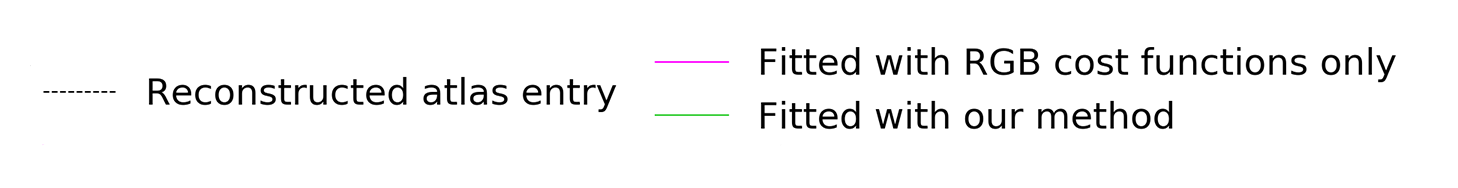
\includegraphics[width=\linewidth]{img/results_costFunctions_legend.png}
	\end{subfigure} \\
	\begin{subfigure}[t]{0.45\textwidth}
		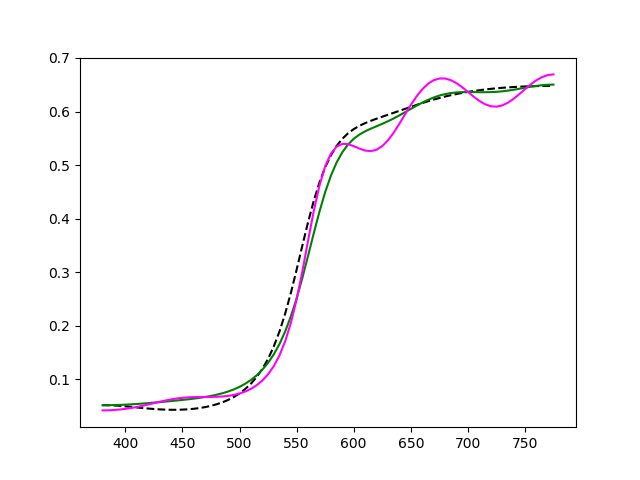
\includegraphics[width=\linewidth]{img/results_costFunctions_orange.png}
		\caption{``orange'' patch of the MCC, $c = 8$, $d = 11.84$}
		\label{fig:resultsCostFunctions_orange}
	\end{subfigure} \hspace{0.1em}
	\begin{subfigure}[t]{0.45\textwidth}
		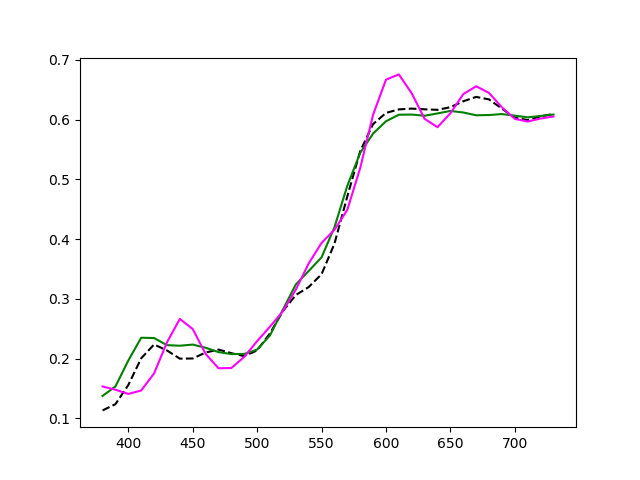
\includegraphics[width=\linewidth]{img/results_costFunctions_mcb0706.png}
		\caption{5YR 7/6 patch of the MBC, $c = 14$, $d = 5.85$}
		\label{fig:resultsCostFunctions_mcb0706}
	\end{subfigure} 
	\vspace{0.5em}\\
	\begin{subfigure}[t]{0.45\textwidth}
		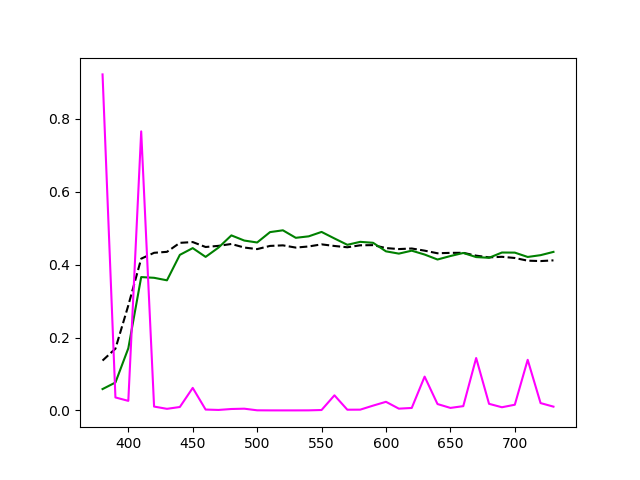
\includegraphics[width=\linewidth]{img/results_costFunctions_mcb0725.png}
		\caption{N 7.25 patch of the MBC, $c = 20$, $d = 12.67$}
		\label{fig:resultsCostFunctions_mcb0725}
	\end{subfigure} \hspace{0.1em}
	\begin{subfigure}[t]{0.45\textwidth}
		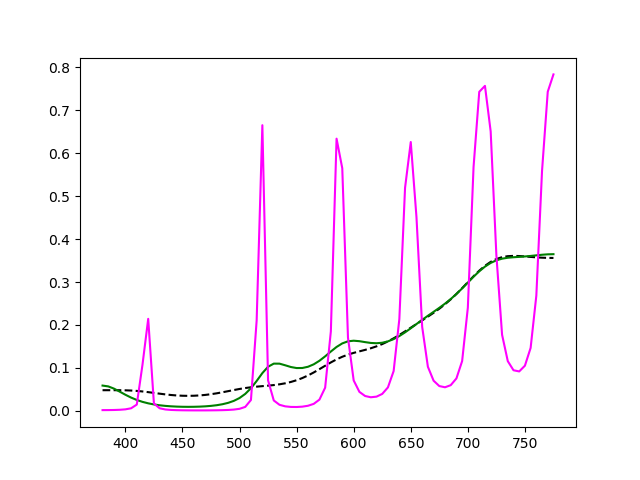
\includegraphics[width=\linewidth]{img/results_costFunctions_darkskin.png}
		\caption{``dark skin'' patch of the MCC, $c = 12$, $d = 11.55$}
		\label{fig:resultsCostFunctions_darkskin}
	\end{subfigure}
	\caption{Comparison between the RGB cost functions and our cost functions for fitting atlas lattice points}
	\label{fig:resultsCostFunctions}
\end{figure}

We therefore conclude that we must incorporate the requirement of curve shape similarity into our cost functions. Following, we review the approaches we attempted along with their outcomes.

The first idea was to implement an approach similar to that for determining the number of coefficients with which to store atlas entries (see~\cref{ssec:noOfMoments}), i.e. to utilize the color error under a fluorescent illuminant (specifically, FL11). We defined three additional cost functions, each specifying the difference between the original and the reconstructed curve's RGB under the FL11 illuminant in one of the axes. If their values fell below a specific threshold, we terminated the fitting process as successful, if not, we increased the threshold and tried again.

Although this approach was successful on average (the average threshold was around $t = 0.025$), occasionally, the threshold often needed to be increased to values so high that it became obsolete (i.e. $t = 1$). Using only one error, either the Euclidean distance or the Delta E error, caused similar issues.

Therefore, we decided to focus on the actual distance between the two curves. Our first attempt consisted of defining one residual per wavelength sample, which specified the absolute distance (as the least square error proved to perform worse) between the two spectra at said wavelength. We examined the behavior of the optimizer both for around 360 residuals (i.e. 1nm increment between samples) and 36 residuals (10nm increment, as defined in most color atlases) when used alongside the 3 already defined RGB residuals. For $c \le 9$, both of these options performed reasonably well, and for $c > 9$ coefficients, the sufficient threshold was, on average, around $t = 0.0096$, for which the curves were fitted quite accurately.

However, although this method definitely outperformed the previous one, it did not completely eliminate the sinusoidal-like artifacts. During our tests, we came across thresholds as high as $t = 0.23$, which definitely needed improvement.

As we suspected that the failures of the optimizer with lower threshold values were caused by the abundance of cost functions, we summed up their values and saved them into a single residual, which, when divided by the number of spectral samples, represented the average absolute error per sample.

As the importance of curve samples in terms of proper color reconstruction is mainly placed on their middle (at around 550nm), we attempted to add a heuristic-based weighting factor in an effort to focus on minimizing the distance between the two curve there. However, we did not succeed in improving our results, and we therefore dropped the experiment and examined the optimizer's behavior without weighting the values.

The proposed method substantially outperformed the previous ones. The threshold error ended up being only about $t = 0.0045$, and, of yet, no entry requiring $d > 0.03$ has been encountered. Therefore, we concluded that the optimal solution to our problem is to set 4 residuals, 3 specifying the RGB difference, and 1 specifying the average distance per sample.

We present some of the results achieved with our cost functions in~\cref{fig:resultsCostFunctions}, where we compare them to fitting with RGB cost functions only. In~\cref{fig:resultsCostFunctions_mcb0725} and~\cref{fig:resultsCostFunctions_darkskin}, we specifically focus on the most problematic spectra with the highest distance $d$ between the atlas lattice point and the atlas entry.

Although our approach substantially reduces the appearance of sinosidual-like behavior, it does not diminish it completely. It can be observed especially for atlas lattice points with $c > 14$ (see~\cref{fig:resultsCostFunctions_mcb0725}). This is due to the fact that we optimize only the first 4 coefficients, which, in their nature, are prone to creating such patterns.

Another drawback of our approach is the substantially greater time complexity, especially if improvement heuristics need to be applied. By examining the scope of the optimizer and utilizing its options further, or maybe even resorting to a different method of optimization, we might be able to improve upon both the time complexity and the resulting spectral shape.

However, as the runtime is not the focus of this thesis and as the resulting shapes are satisfactory for the purposes of accurate uplifting, we leave these improvements for future work.

\section{Colorimetric properties}

In the following, we evaluate the accuracy of our technique when used for uplifting constraints and compare its results to the sigmoid-based uplift as defined by~\citet{upsamplingJakobHanika}. We then assess its performance when uplifting the RGB gamut as a whole.

All the data of color atlases and illuminants used in our experiments is provided by ART~\cite{ART}.

\begin{figure}[ht!]
	\centering
	{\sffamily
		\setlength\tabcolsep{0.0pt}
		%\renewcommand{\arraystretch}{0.1}
		\begin{tabular}{ccccccc}
			&Original& Uplifted & Difference &\quad Original & Uplifted & Difference
			\vspace{1em} \\ 
			\raisebox{0.4cm}[0pt][0pt]{\parbox[c][0pt][c]{0cm}{\hspace{-1.5em}\rotatebox{90}{Sigmoid}\\[20pt]}\par}
			&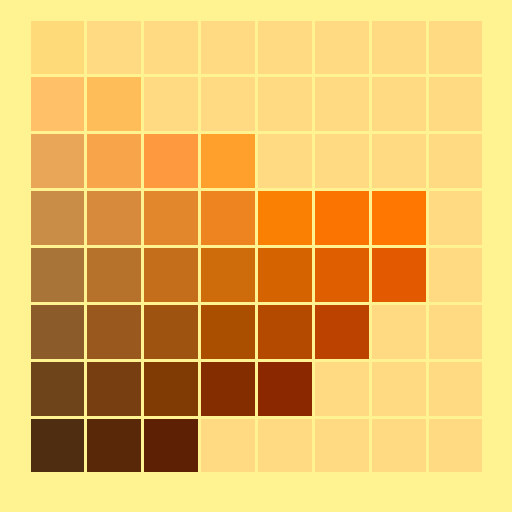
\includegraphics[width=.15\linewidth]{img/results_uplift_page04_originalFL3.png}
			&
			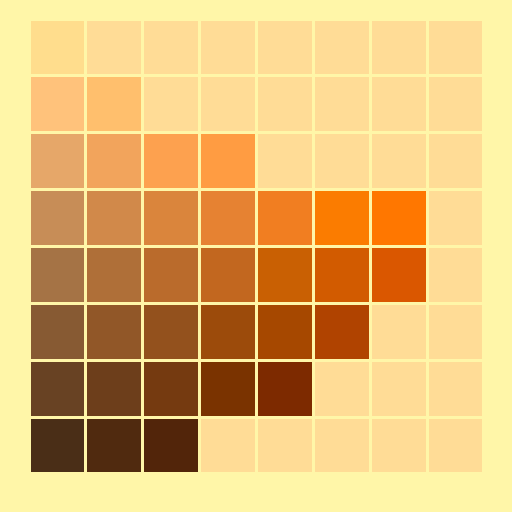
\includegraphics[width=.15\linewidth]{img/results_uplift_page04_sigmoidFL3.png}
			& 
			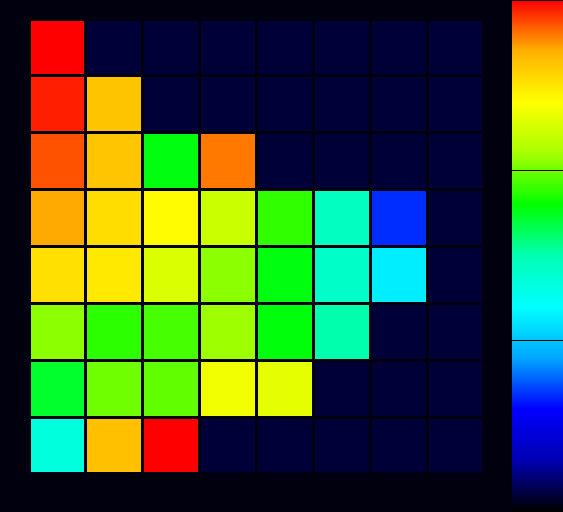
\includegraphics[width=.15\linewidth,height=5.25em]{img/results_uplift_page04_diff_sigmoidFL3.png}
			&\quad
			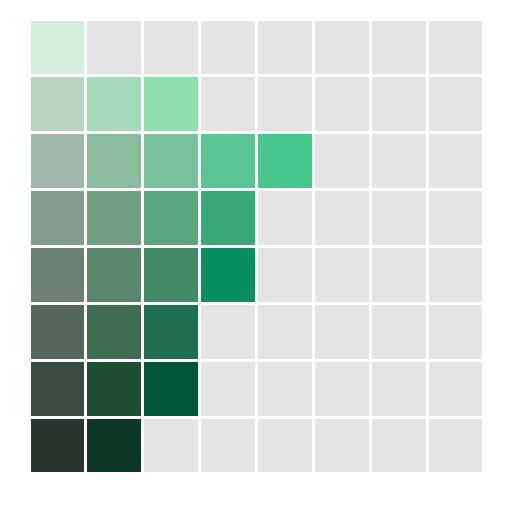
\includegraphics[width=.15\linewidth]{img/results_uplift_page18_originalD65.png}
			&
			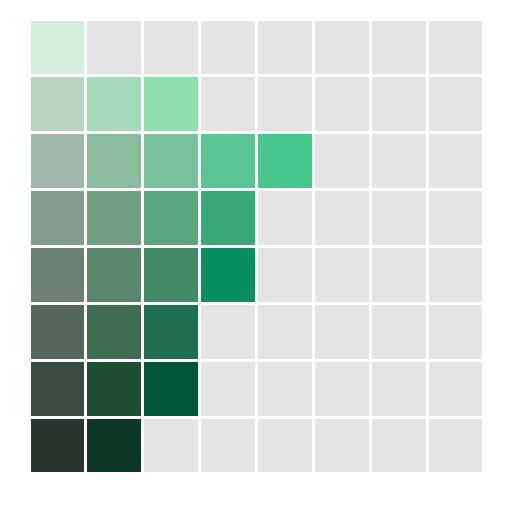
\includegraphics[width=.15\linewidth]{img/results_uplift_page18_sigmoidD65.png}
			&
			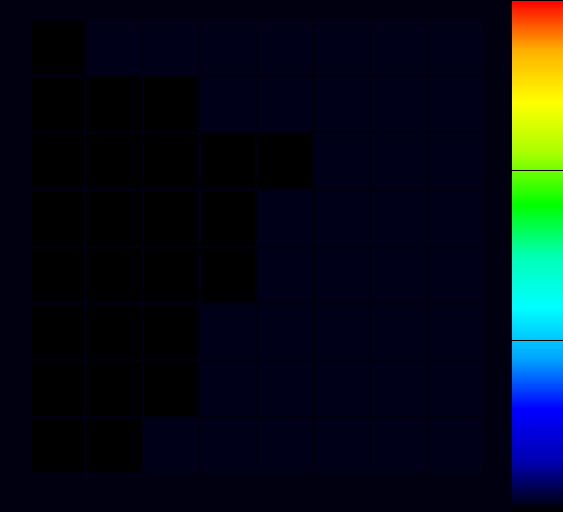
\includegraphics[width=.15\linewidth,height=5.25em]{img/results_uplift_page18_diff_sigmoidD65.png}
			\\ \raisebox{0.5cm}[0pt][0pt]{\parbox[c][0pt][c]{0cm}{\hspace{-1.5em}\rotatebox{90}{Our}\\[20pt]}\par}
			&
			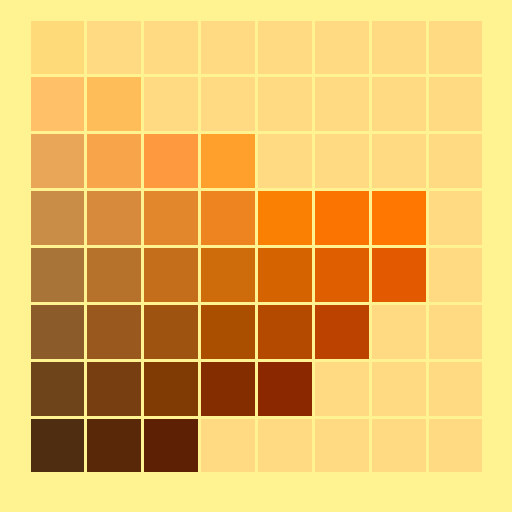
\includegraphics[width=.15\linewidth]{img/results_uplift_page04_originalFL3.png}
			&
			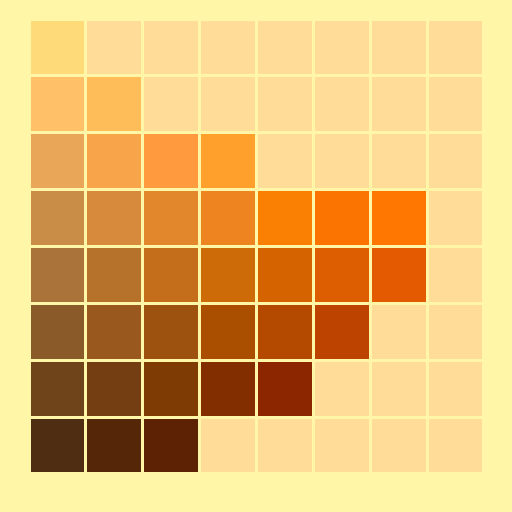
\includegraphics[width=.15\linewidth]{img/results_uplift_page04_ourFL3.png}
			& 
			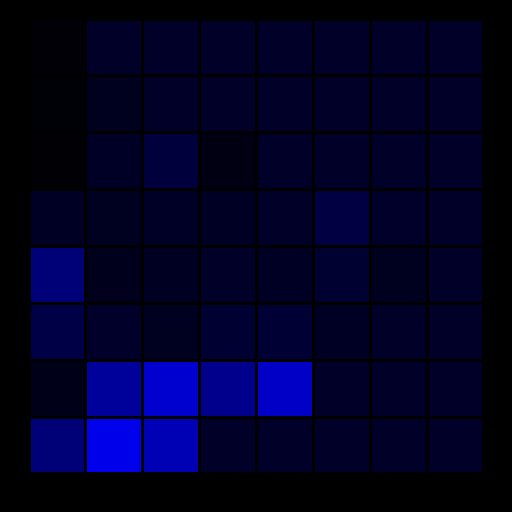
\includegraphics[width=.15\linewidth,height=5.25em]{img/results_uplift_page04_diff_ourFL3.png}
			&\quad
			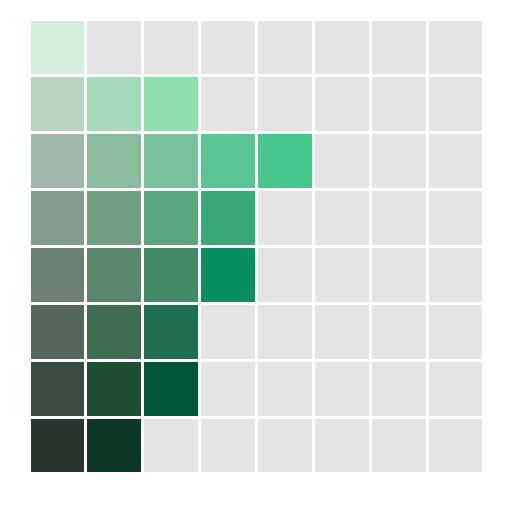
\includegraphics[width=.15\linewidth]{img/results_uplift_page18_originalD65.png}
			&
			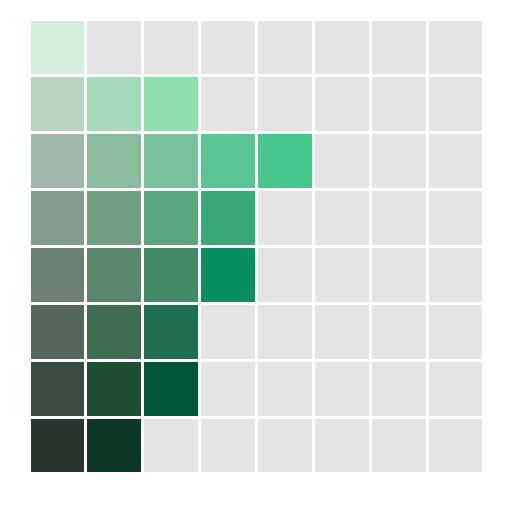
\includegraphics[width=.15\linewidth]{img/results_uplift_page18_ourD65.png}
			&
			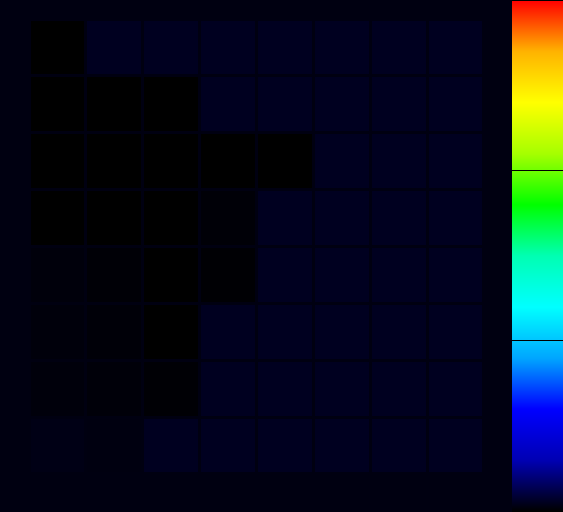
\includegraphics[width=.15\linewidth,height=5.25em]{img/results_uplift_page18_diff_ourD65.png}\\
			& & Page 4; FL 3 & & & Page 18; D65 & \\
			\vspace{0.1em} \\ 
			\raisebox{0.4cm}[0pt][0pt]{\parbox[c][0pt][c]{0cm}{\hspace{-1.5em}\rotatebox{90}{Sigmoid}\\[20pt]}\par}
			&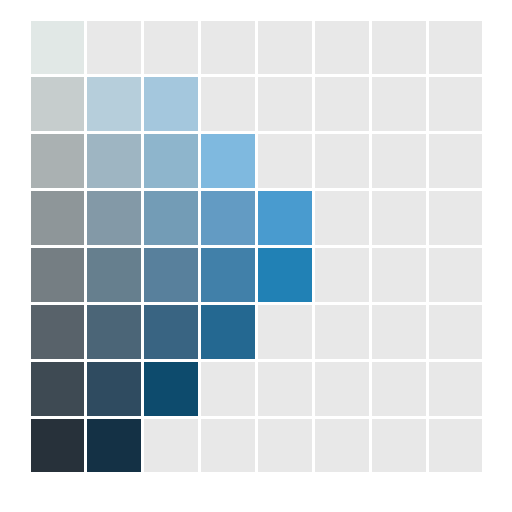
\includegraphics[width=.15\linewidth]{img/results_uplift_page29_originalFL7.png}
			&
			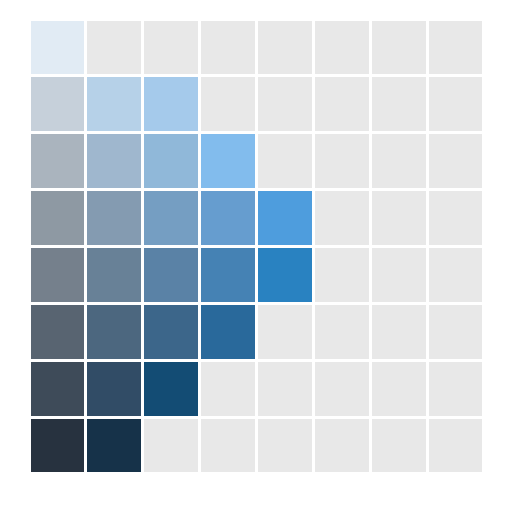
\includegraphics[width=.15\linewidth]{img/results_uplift_page29_sigmoidFL7.png}
			& 
			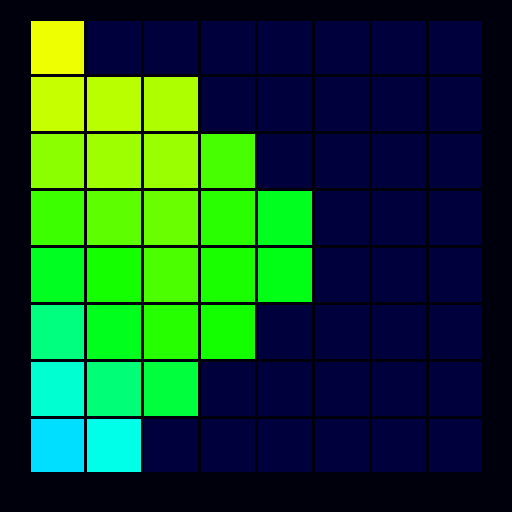
\includegraphics[width=.15\linewidth,height=5.25em]{img/results_uplift_page29_diff_sigmoidFL7.png}
			&\quad
			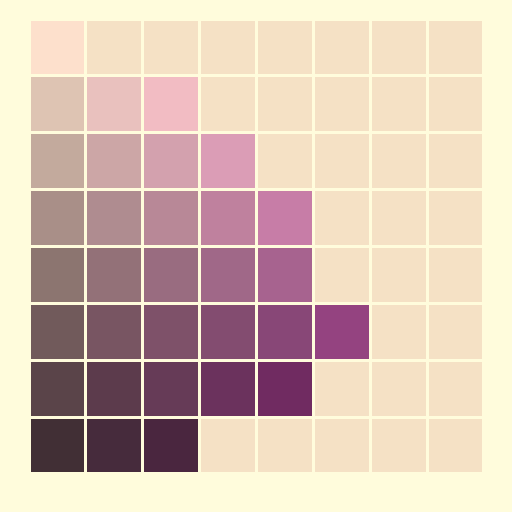
\includegraphics[width=.15\linewidth]{img/results_uplift_page35_originalD50.png}
			&
			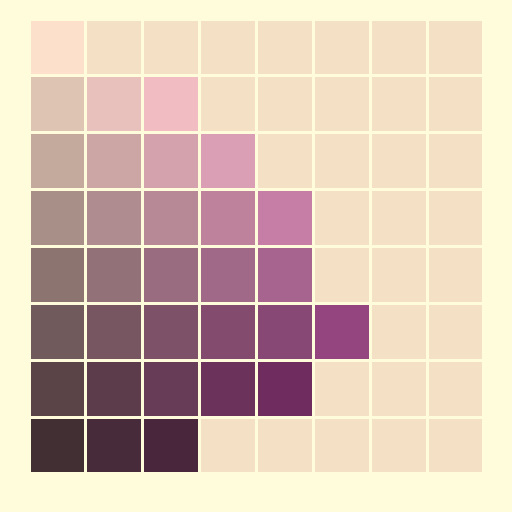
\includegraphics[width=.15\linewidth]{img/results_uplift_page35_sigmoidD50.png}
			&
			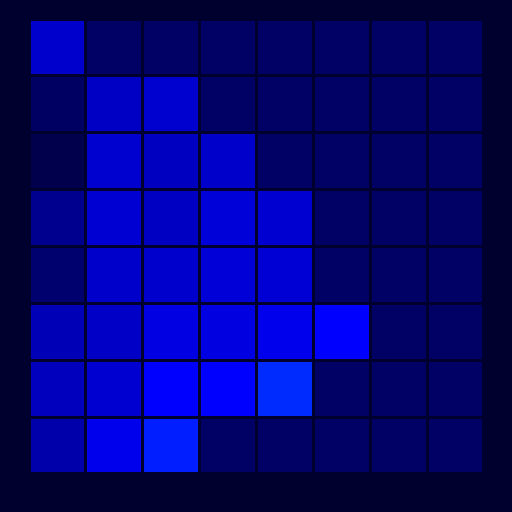
\includegraphics[width=.15\linewidth,height=5.25em]{img/results_uplift_page35_diff_sigmoidD50.png}
			\\ \raisebox{0.5cm}[0pt][0pt]{\parbox[c][0pt][c]{0cm}{\hspace{-1.5em}\rotatebox{90}{Our}\\[20pt]}\par}
			&
			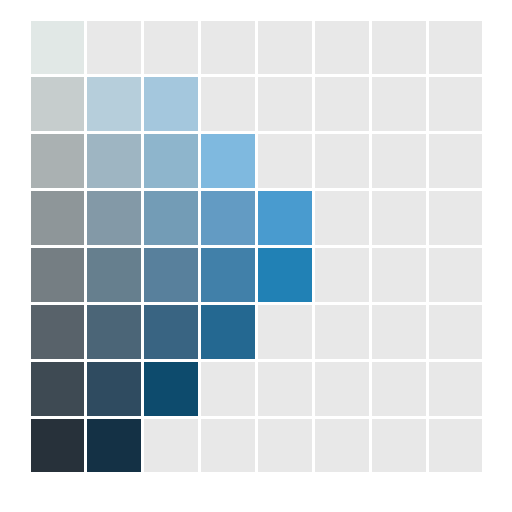
\includegraphics[width=.15\linewidth]{img/results_uplift_page29_originalFL7.png}
			&
			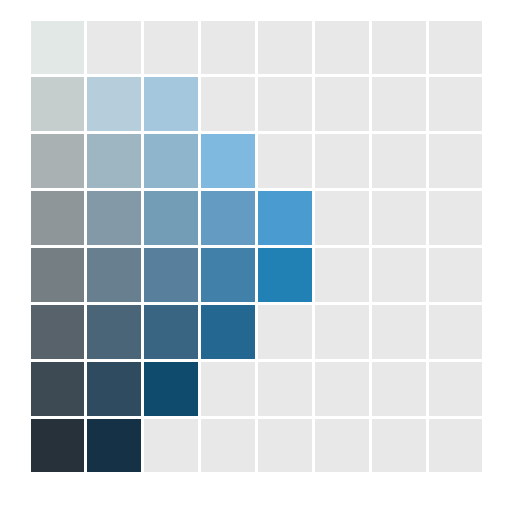
\includegraphics[width=.15\linewidth]{img/results_uplift_page29_ourFL7.png}
			& 
			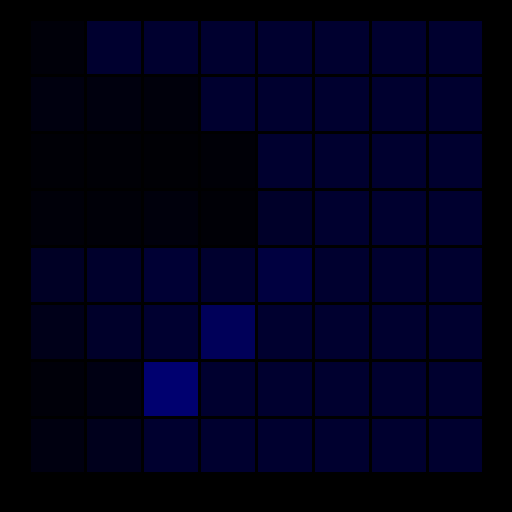
\includegraphics[width=.15\linewidth,height=5.25em]{img/results_uplift_page29_diff_ourFL7.png}
			&\quad
			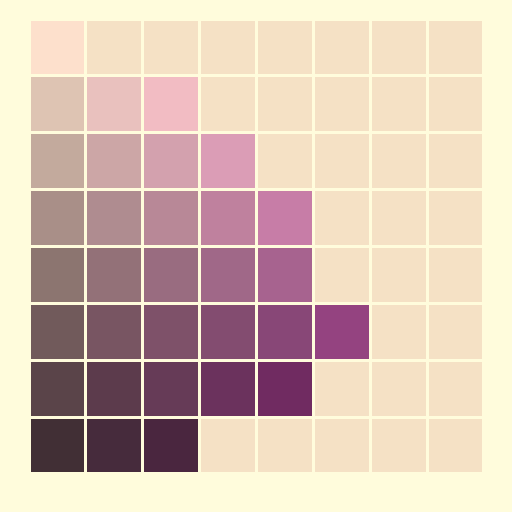
\includegraphics[width=.15\linewidth]{img/results_uplift_page35_originalD50.png}
			&
			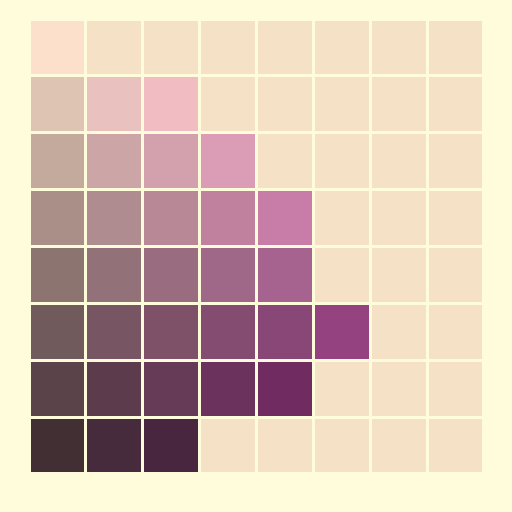
\includegraphics[width=.15\linewidth]{img/results_uplift_page35_ourD50.png}
			&
			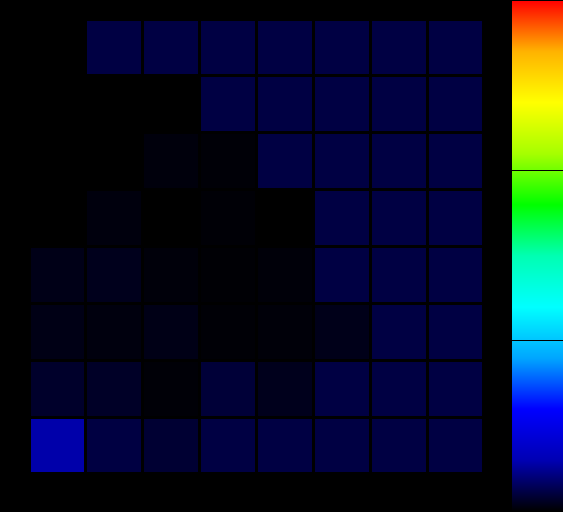
\includegraphics[width=.15\linewidth,height=5.25em]{img/results_uplift_page35_diff_ourD50.png}\\
			& & Page 29, FL 7 & & & Page 35, D50 & \\
			\vspace{0.1em} \\ 
			\raisebox{0.4cm}[0pt][0pt]{\parbox[c][0pt][c]{0cm}{\hspace{-1.5em}\rotatebox{90}{Sigmoid}\\[20pt]}\par}
			&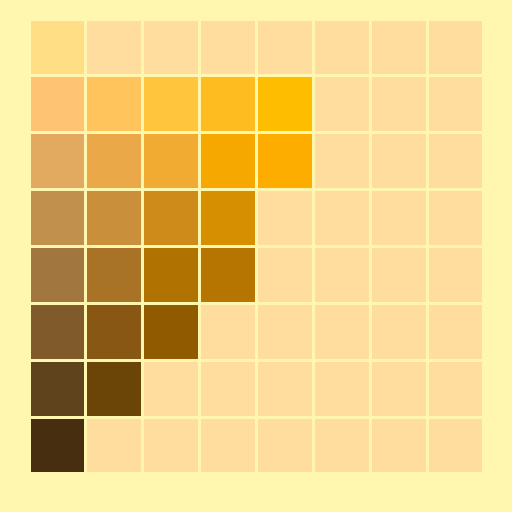
\includegraphics[width=.15\linewidth]{img/results_uplift_page09_originalFL11.png}
			&
			\includegraphics[width=.15\linewidth]{img/results_uplift_page09_sigmoidFL11.png}
			& 
			\includegraphics[width=.15\linewidth,height=5.25em]{img/results_uplift_page09_diff_sigmoidFL11.png}
			&\quad
			\includegraphics[width=.15\linewidth]{img/results_uplift_page14_originalFL11.png}
			&
			\includegraphics[width=.15\linewidth]{img/results_uplift_page14_sigmoidFL11.png}
			&
			\includegraphics[width=.15\linewidth,height=5.25em]{img/results_uplift_page14_diff_sigmoidFL11.png}
			\\ \raisebox{0.5cm}[0pt][0pt]{\parbox[c][0pt][c]{0cm}{\hspace{-1.5em}\rotatebox{90}{Our}\\[20pt]}\par}
			&
			\includegraphics[width=.15\linewidth]{img/results_uplift_page09_originalFL11.png}
			&
			\includegraphics[width=.15\linewidth]{img/results_uplift_page09_ourFL11.png}
			&
			\includegraphics[width=.15\linewidth,height=5.25em]{img/results_uplift_page09_diff_ourFL11.png}
			&\quad
			\includegraphics[width=.15\linewidth]{img/results_uplift_page14_originalFL11.png}
			&
			\includegraphics[width=.15\linewidth]{img/results_uplift_page14_ourFL11.png}
			&
			\includegraphics[width=.15\linewidth,height=5.25em]{img/results_uplift_page14_diff_ourFL11.png}\\
			& & Page 09, FL 11 & & & Page 14, FL 11 & \\
		\end{tabular}
	}
	\caption{Comparison of our uplifting model with the sigmoid-based technique~\cite{upsamplingJakobHanika} for pages of the Munsell Book of Color under different illuminants. Maximum Delta E in the difference images is 3. Note that patches that fall outside sRGB have been omitted.}
	\label{fig:results_uplift_munsell}
\end{figure}


\subsection{Constraint uplifting accuracy}

We tested the accuracy of our proposed constrained uplifting approach on the Munsell Book of Color (MBOC), which we utilized as a constraint set for a $32^3$-sized coefficient cube for the sRGB color space. Of the 1598 entries in the MBOC, 1396 are in the sRGB gamut: therefore, our experiments only included those. If a larger RGB space (such as e.g. Adobe RGB) were used as input space, the full number of atlas entries could be used: working with sRGB was not due to any restrictions in our proposed technique, but only done to stay within the standard RGB space of graphics. Furthermore, in a $32^3$-sized coefficient cube, 82 of the atlas entries can not be used as seeds due to the limitation that only one seed can be present in each voxel. Simply increasing the cube resolution would allow to use the 82 missing entries: again, using a $32^3$ coefficient cube was not done due to any intrinsic restrictions of our technique, but just to save pre-computation time, and stay with a nice power of two as cube dimension.

We compared the difference between the uplifted spectra to the original ones under a spiky, error-prone illuminant via the standard CIE Delta E color difference metric. Specifically, we present the results under the FL11 illuminant, as we determined it to be the illuminant most susceptible to metameric failures (from the ART databse) --- under D65, the error was negligible throughout the whole spectrum.

The average round-trip error was just a Delta E of $0.21$. As the maximum error perceivable by a standard observer is $\Delta E<1$~\cite{maxColorDifference}, this value is negligible and can be regarded as highly satisfactory. Of the 1314 entries, only 22 were found to return a $\Delta E > 1$: all of these were RGB values extremely close to $(0,0,0)$. 

\begin{figure}[t!]
	\centering
	\includegraphics[width=0.6\linewidth]{img/seeding_accuracy_legend.png}
	\includegraphics[width=0.45\linewidth]{img/seeding_accuracy_dark_12coef.png}
	\includegraphics[width=0.45\linewidth]{img/seeding_accuracy_dark_14coef.png}
	\caption{Problematic cases of constrained uplifting: reflectance spectra of darker colors. In the areas where the round-trip plot is barely visible, it mimics the original spectrum. Note that the demonstrated range on the y-axis is not $[0,1]$.}
	\label{fig:seeding_accuracy_dark}
\end{figure}

An example of this behavior in the dark region of the RGB cube can be observed in~\cref{fig:results_uplift_munsell}. The reason for it is the inadequate fitting of seeded points by the optimizer. This behavior was already present in~\cref{ssec:costFunctions} in~\cref{fig:resultsCostFunctions}, where we concluded that it is due to both the moment representation's inability to flawlessly reconstruct constant curves, and the optimizer's tendency to amplify this deficiency. As the spectral shapes of the dark colors resemble almost constant lines close to zero, it makes sense that the optimiser would primarily fail there.

In~\cref{fig:seeding_accuracy_dark} and~\cref{fig:seeding_accuracy_other}, we provide comparisons of curves of the original spectra, the seeded spectra (labeled \emph{round-trip}, i.e. it represents the direct reconstruction from the moments used to store the original spectra) and the uplifted spectra (i.e. the result of querying the final coefficient cube, including interpolation within the voxel the RGB value lies in). Ideally, all three curves should be identical: a difference between ``original'' and ``round-trip'' points to the deficiency of the moment-based spectral reconstruction, while a difference between ``round-trip'' and ``uplift'' indicates a drawback in the optimizer. We can observe that, while for darker colors (see~\cref{fig:seeding_accuracy_dark}), the errors are mainly due to inadequacies of the optimizer, slight curve deviations for brighter colors (see~\cref{fig:seeding_accuracy_other}) are usually due to imperfections of the moment representation.

\begin{figure}[ht]
	\centering
	\includegraphics[width=0.6\linewidth]{img/seeding_accuracy_legend.png}
	\includegraphics[width=0.45\linewidth]{img/seeding_accuracy_6coef.png}
	\includegraphics[width=0.45\linewidth]{img/seeding_accuracy_12coef.png}
	\vspace{0.5em}\\
	\includegraphics[width=0.45\linewidth]{img/seeding_accuracy_15coef.png}
	\includegraphics[width=0.45\linewidth]{img/seeding_accuracy_19coef.png}
	\caption{Accuracy of constrained uplifting demonstrated on examples of input spectra that correspond to saturated RGB colors. In the areas where the round-trip plot is barely visible, it mimics the uplifted spectrum.}
	\label{fig:seeding_accuracy_other}
	\vspace{-1em}
\end{figure}

However, neither of the mentioned deficiencies severely degrade the accuracy of the uplifting system. On the contrary --- in~\cref{fig:results_uplift_munsell}, we can clearly observe our contribution. While the images uplifted with the sigmoid-based cube demonstrate rather significant color errors, our uplifting system performs modestly and is, except for slight, barely visible discrepancies, almost identical to the original spectral render.

Unfortunately, we have encountered issues when testing the accuracy of our system in a conventional spectral renderer (specifically, ART~\cite{ART}). Due to minor color deviations that arise during spectral rendering, the RGB values directly evaluated from the input spectra are not generally equal to the RGB values outputted in the rendered texture. Although the differences are negligible in terms of human color perception, they are high enough to cause the two values to fall into different cube voxels (specifically, to cause the texture RGB to fall into a non-seeded voxel), which in turn results in the insufficient uplift of the texture RGB.

For this reason, in order to demonstrate the correctness of our model on an example scene in~\cref{fig:results_art_scene}, we do not use the spectrally rendered textures but rather our own, manually-created, which perfectly match the desired RGB values. As the method was not tested in other renderers, we attribute the need for such a process to the inaccuracy of ART. 

\begin{figure}[ht]
	\centering
	{\sffamily
		\begin{tabular}{cccc}
			Spectral render & Sigmoid uplift & Our uplift
			\vspace{1em} \\
			\raisebox{0.5cm}[0pt][0pt]{\parbox[c][0pt][c]{0cm}{\hspace{-1.5em}\rotatebox{90}{D65}\\[10pt]}\par}
			\includegraphics[width=.29\linewidth]{img/results_art_original_d65.png}
			&
			\includegraphics[width=.29\linewidth]{img/results_art_sigmoids_d65.png}
			& 
			\includegraphics[width=.29\linewidth]{img/results_art_constrained_d65.png}
			\vspace{1em} \\
			\raisebox{0.5cm}[0pt][0pt]{\parbox[c][0pt][c]{0cm}{\hspace{-1.5em}\rotatebox{90}{FL12}\\[10pt]}\par}
			\includegraphics[width=.29\linewidth]{img/results_art_original_fl12.png}
			&
			\includegraphics[width=.29\linewidth]{img/results_art_sigmoids_fl12.png}
			&
			\includegraphics[width=.29\linewidth]{img/results_art_constrained_fl12.png}
		\end{tabular}
	}
	\caption{Comparison of the sigmoid-based uplift to the constrained uplift on a scene rendered in ART~\cite{ART}. Pages in scene are (from the left): 050Y, 050GY, 100Y.}
	\label{fig:results_art_scene}
\end{figure}

\subsection{Uplift consistency across RGB Space}

In order to assess how our technique uplifts the entire RGB gamut (and not just the regions around the seeds), we created multiple coefficient cubes that were seeded with different color atlases. This included a non-constrained cube, i.e. a cube fitted from the middle point at $\mathrm{RGB}(0.5,0.5,0.5)$ in the same manner as the sigmoid-based approach by Jakob and Hanika~\cite{upsamplingJakobHanika}). 

We first compared their performance in terms of color reconstruction upon uplifting a gradient texture. We specifically selected a gradient with saturated colors in the red-yellow-green region, as that is where differences are most perceivable. The results are shown in~\cref{fig:colorimetric_properties}, again illuminated by CIE FL11 (under D65, there are, as per the fitting process, practically zero differences). While the distinctions between individual uplifts under FL11 are barely perceivable by the human eye, the difference images demonstrate that there are some variations -- mainly around the locations of seed points, which is precisely what is intended by constraining the uplift process in these locations. None of the gradient textures exhibit any visible discontinuities, though, which indicates that our interpolation approach works properly in the presence of multiple metameric families of reflectance spectra.

\begin{figure}[t]
	\centering
	{\sffamily
		\setlength\tabcolsep{1.5pt}
		\begin{tabular}{ccccc}
			&\makecell{Uplifted\\with\\sigmoids}&\quad \makecell{Munsell Book\\of\\Colors}& \quad
			\makecell{\\None\\}&\quad \makecell{Pantone\\Color\\System}
			\vspace{1em} \\ 
			\raisebox{1.5em}[0pt][0pt]{\parbox[c][0pt][c]{0cm}{\hspace{-1.5em}\rotatebox{90}{Uplift}\\[18pt]}\par}
			&
			&\quad
			\includegraphics[width=.20\linewidth]{img/gradient_uplift_mbc.png}
			& \quad
			\includegraphics[width=.20\linewidth]{img/gradient_uplift_middle.png}
			& \quad
			\includegraphics[width=.20\linewidth]{img/gradient_uplift_pantone.png}
			\\ \raisebox{1.5em}[0pt][0pt]{\parbox[c][0pt][c]{0cm}{\hspace{-1.5em}\rotatebox{90}{Difference}\\[18pt]}\par}
			&
			\includegraphics[width=.20\linewidth]{img/gradient_uplift_sigmoid.png}
			& \quad
			\includegraphics[width=.20\linewidth, height=7em]{img/gradient_diff_mbc.png}
			& \quad
			\includegraphics[width=.20\linewidth, height=7em]{img/gradient_diff_middle.png}
			& \quad
			\includegraphics[width=.20\linewidth, height=7em]{img/gradient_diff_pantone.png}\\
		\end{tabular}
	}
	\caption{A region of the RGB gamut uplifted with different sets of initial spectra, illuminated by FL11. The difference images are relative to maximum $\Delta E = 2$.}
	\label{fig:colorimetric_properties}
	\vspace{-1em}
\end{figure}

In~\cref{fig:uplift_colourful_texture}, we demonstrate that our approach can properly uplift large regions of the RGB gamut simultaneously, without showing artifacts under varying illuminations. We provide multiple uplifts of a rainbow texture covering most of the RGB gamut, constrained with different constraint sets under various illuminants. Although a significant subset of voxels has been seeded, some of them with spiky spectra (especially for the Pantone color atlas), none of these renderings exhibits significant artifacts. Note that all uplifts were performed with $32^3$-sized cubes, i.e. some of the constraints may not have been utilized due to collisions during seeding.

\begin{figure}[ht]
	\centering
	{\sffamily
		\setlength\tabcolsep{1.5pt}
		\begin{tabular}{cccc}
			\makecell{Original\\D65} & \makecell{MBOC\\D50} & \makecell{Pantone\\FL5} &\makecell{RAL\\FL12}
			\vspace{0.5em}\\ 
			\includegraphics[width=.22\linewidth]{img/gradient_complete.jpg}
			&
			\includegraphics[width=.22\linewidth]{img/gradient_complete_mbcD50.jpg}
			& 
			\includegraphics[width=.22\linewidth]{img/gradient_complete_pantoneFL5.jpg}
			& 
			\includegraphics[width=.22\linewidth]{img/gradient_complete_ralFL12.jpg} \vspace{0.5em}\\
			\makecell{Pantone\\D75}& \makecell{None\\FL9} & \makecell{RAL\\FL7}  & \makecell{MCC SG\\FL3}
			\vspace{0.3em}\\
			\includegraphics[width=.22\linewidth]{img/gradient_complete_pantoneD75.jpg}
			&
			\includegraphics[width=.22\linewidth]{img/gradient_complete_noneFL9.jpg}
			& 
			\includegraphics[width=.22\linewidth]{img/gradient_complete_ralFL7.jpg}
			& 
			\includegraphics[width=.22\linewidth]{img/gradient_complete_mccSGFL3.jpg}\\
		\end{tabular}
	}
	\caption{Constrained spectral uplifting of a colorful texture for various constraint sets under different illuminants.}
	\label{fig:uplift_colourful_texture}
	\vspace{-1em}
\end{figure}


\section{Performance and future work}

In this section, we evaluate the performance of our method in terms of both memory and execution time, and propose possible future work for their improvement.

\subsection{Memory usage}
The memory necessary for storing our cube depends on its resolution (i.e. the number of lattice points), which is, in turn, dependent on both the size of our constraint set and on the position of its spectra within the RGB cube. The Macbeth Color Checker (MCC), which contains only 24 entries that are spaced quite far apart from each other in the RGB space (with one of them falling outside of sRGB), requires as little as a $13^3$-sized cube. Due to the close proximity of some seeds, the 1396 sRGB entries of the Munsell Book of Color would require as much as 340 lattice points per axis for all seeds to fall into a unique voxel. Additionally, due to the rigid nature of an evenly spaced voxel grid, using a higher cube dimension does not necessarily imply more points that can be successfully seeded. Due to voxel edges being in different positions for different cube dimensions, increasing cube size might even have an adverse effect --- for example, while a cube of size $90^3$ is sufficient for the RAL Design atlas, in a $300^3$-sized cube, 1 point remains unfitted due to a voxel collision.

To store the coefficients of cube entries, we require 3 floating point values for all non-seeded points, and, on average, 16 floating point values per constraint. For the $340^3$-sized cube required for the proper coverage of the Munsell Book of Color, this would yield a size of over $450.35$MB. Although using less coefficients for storing constraints is possible, it would not noticeably improve the size of the cube --- even if we were to use 3 coefficients for all coefficient representations within the cube, the overall size would still be over $449.8$MB. That is a negligible improvement, as the overall size remains excessive --- after all, a seeding of the whole Munsell Book of Color requires only $1396$ voxels, which sums up to a maximum of $8\cdot1396$ lattice points. Additionally, while most of the regions of the cube are barely utilized, there exist some that have all of their voxels fitted, which might result in a lack of smooth color transitions within these regions.

We therefore conclude that, for the purposes of constrained spectral uplifting for large sets of user-supplied target spectra (like e.g. entire color atlases), a coefficient cube with evenly spaced lattice points is distinctly sub-optimal, in terms of both the memory requirements and its resulting colorimetric properties. For future work, we suggest utilizing a dynamic structure capable of splitting the RGB space into variably-sized voxels according to the number of constraints, such as a kD-tree or an octree.

\subsection{Execution time}

Since our uplifting model is created prior to the rendering process, we divide the evaluation of the execution time into two parts --- the cube fitting process, and the rendering speed when utilizing our cube for uplifting purposes.

We test the execution time of cube fitting on multiple sets of constraints in forms of color atlases, and present the results in~\cref{fig:evaluation_cube_fitting}, where we distinguish the \emph{seeding time} (i.e. the time spent on seeding and fitting of the atlas lattice points) and the \emph{fitting time} (i.e. the time spent on fitting the rest of the cube, i.e. the regular lattice points). All the experiments are performed on an Intel Core i7-8750H CPU (12 logical cores), and the size of each cube is $32^3$. Note that such cube resolution may be insufficient for the utilization of all constraints in a given atlas --- we therefore provide the \emph{seed count}, which represents the overall number of moment representations stored at atlas lattice points.

\begin{table}[h]
	\centering
	\begin{tabular}{ lrrrr } 
		\hline
		\noalign{\vskip 0.3em}   
		\makecell{Color\\atlas} & \makecell{Seed\\count} & \makecell{Seeding\\time} & \makecell{Fitting\\time} & Overall \vspace{0.3em} \\
		\hline
		\noalign{\vskip 0.3em}   
		Munsell Book of Color& 10512 		&7h 32m 18s&6m 59s &7h 39m 17s\\ 
		RAL Design Atlas & 1336		&43m 11s&9m 15s &52m 26s\\ 
		Macbeth Color Chart SG	& 576	&27m 14s&8m 8s  &35m 22s\\ 
		Macbeth Color Chart& 184 		&9m 29s &14m 17s&23m 46s\\ 
		None & 1 		&0.08s&45m 5s &45m 6s\\
		Sigmoid-based approach	&1 &0s&7m 16s &7m 16s\\
		\hline
	\end{tabular}
	\caption{Fitting time of a $32^3$-sized coefficient cube for multiple color atlases.}
	\label{fig:evaluation_cube_fitting}
	\vspace{-1em}
\end{table}

Due to the higher coefficient count and the strict requirements placed upon the shapes of the reconstructed spectral curves, the fitting of the atlas lattice points takes a lot longer than the fitting of the latter (on average, an atlas lattice point point takes $2.4$ seconds to fit, in comparison to the $0.03$ for regular lattice points). However, as the cube fitting process is multi-threaded, it benefits from multiple seeds evenly positioned across the RGB cube. This is particularly obvious when comparing the performance of the fitting of the Macbeth Color Charts and the fitting without constraints.

None of these usage cases outperform the sigmoid-based cube in terms of fitting time. While our technique needs to use various complex mathematical operations, such as the application of Levinson's algorithm, Herglotz transform and multiple other conversion processes~\cite{trigonometricMomentsPaper}, not to mention the interpolation of metamers for lattice points with multiple representations, the sigmoid-based approach evaluates the spectral curve with as little as six floating point operations for any given wavelength~\cite{upsamplingJakobHanika}.

This drawback of our technique also carries over to using our method during rendering. In order to properly evaluate the execution time, we perform two tests --- firstly, we compare the performance of the sigmoid-based cube with the performance of our non-constrained cube (in order to avoid the overhead of spectral reconstruction from higher-dimensional coefficient representations), and secondly, we provide measures of the execution time of the constrained uplift of the renders in~\cref{fig:results_uplift_munsell}. All experiments are performed on an Intel Xeon CPU E5-2680 v3 (48 logical cores), with $32^3$-sized cubes.

For the latter experiments, the sigmoid-based approach performed, on average, $2.1$ times better than our constrained cubes. The performance overhead arising from constraining the uplifting process was expected. When used in a spectral renderer -- specifically, ART~\cite{ART} --- on a closely viewed texture of one of the pages of the Munsell Book of Color (that is, when pretty much all the pixels in the image correspond to the constraints), rendering times slow down by about a factor of $4$ when compared to the sigmoid uplift.

For non-constrained uplifting, our method provides no benefits compared to the sigmoid-based approach, except perhaps that it creates slightly more varied spectral shapes than the plain sigmoid technique. Even when not constrained, uplifting of the colorful textures shown in~\cref{fig:uplift_colourful_texture} is $2.3$ times slower with our cube than with the sigmoid-based technique.

That having been said, we wish to point out that so far, our focus was placed on the correctness and accuracy of the constrained uplift, i.e. our implementation of both the model creation and its utilization in a renderer does not include any real optimizations yet. In the future, these could be applied to the fitting process (by further exploiting the possibilities of the CERES solver, or, possibly, another optimization technique) and to the actual uplifting, which currently does not cache any intermediate values (such as the exponential moments) and therefore requires them to be unnecessarily re-computed during each uplift. We estimate that such optimizations could improve the performance up to a factor of two, both during fitting, and during rendering.